\documentclass{beamer}

% For more themes, color themes and font themes, see:
% http://deic.uab.es/~iblanes/beamer_gallery/index_by_theme.html
%
\mode<presentation>
{
  \usetheme{Madrid}       % or try default, Darmstadt, Warsaw, ...
  \usecolortheme{beaver} % or try albatross, beaver, crane, ...
  \usefonttheme{serif}    % or try default, structurebold, ...
  \setbeamertemplate{navigation symbols}{}
  \setbeamertemplate{caption}[numbered]
} 

\usepackage{tikz}
\usetikzlibrary{decorations.markings,angles}
				\usepackage{tikz-3dplot} 

\usepackage{amsmath}

\begin{document}

\title[Two-fluid simulations]  
{Two-fluid simulations of waves and reconnection with Mancha code}
\author[]{Beatrice Popescu Braileanu, \'Angel de Vicente, Elena Khomenko }
\date{September 1, 2016}

\begin{frame}
\maketitle
\end{frame}

\begin{frame}[t]{Solar atmospheric layers}
\vspace*{-22pt}
\begin{columns}[b]
    \begin{column}{0.6\textwidth}
		Photosphere
        \begin{itemize}
					\item collision dominated: LTE, MHD 
					\item	relatively easy observations 
					\item	diagnostics techniques well developed 
        \end{itemize}
    \end{column}
    
    \begin{column}{0.5\textwidth}
       % \rule{\textwidth}{0.75\textwidth}
			\begin{figure}[t]
			 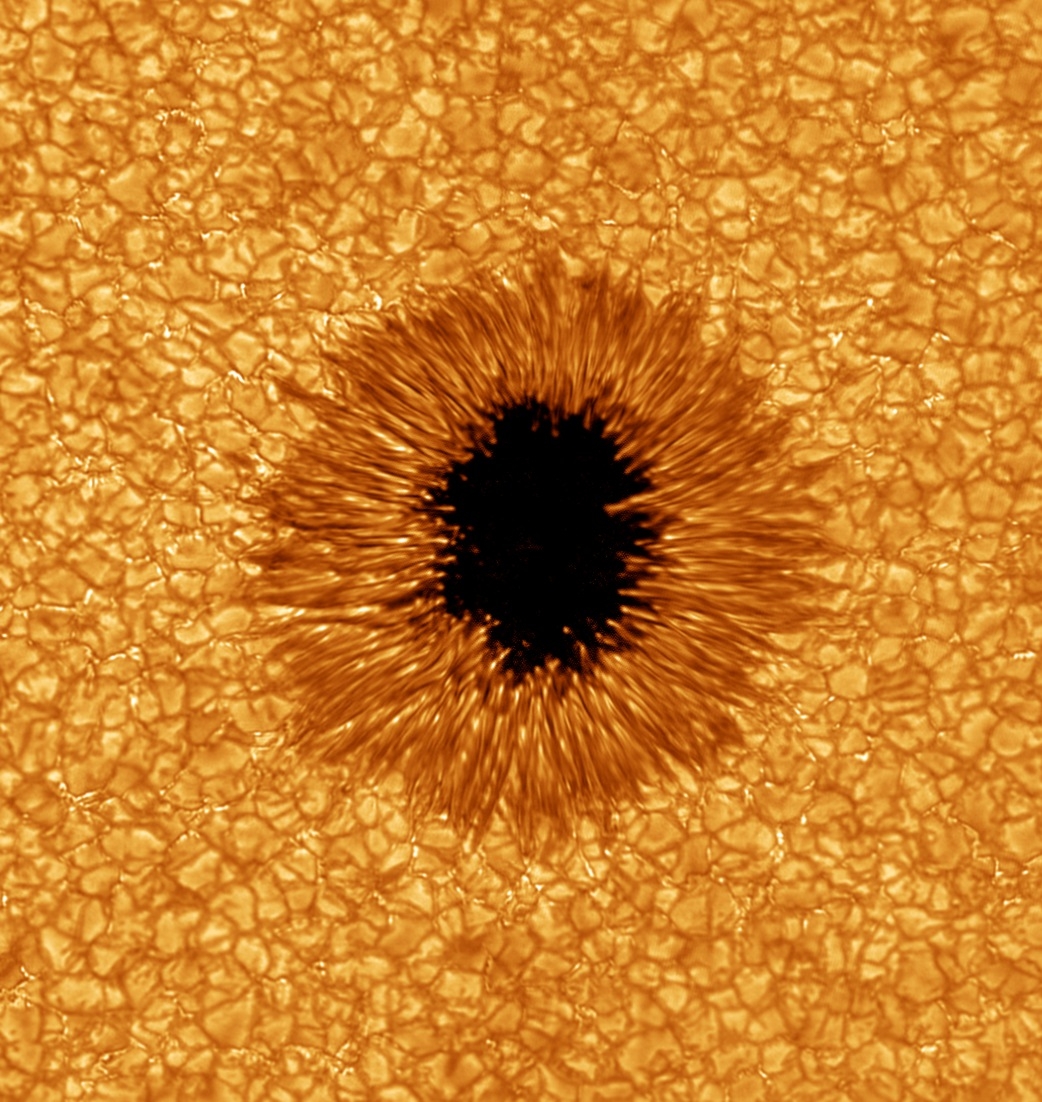
\includegraphics[scale=0.08]{phot.jpg}
			\end{figure}
    \end{column}
\end{columns} 

\vspace{0.1cm}
\begin{columns}[b]
    \begin{column}{0.6\textwidth}
		Chromosphere
        \begin{itemize}
					\item not fully collisionally coupled: NLTE, No MHD (frequently not taken into account)
					\item very few spectral lines 
					\item complicated radiative diagostics 
        \end{itemize}
    \end{column}
    \begin{column}{0.5\textwidth}
       % \rule{\textwidth}{0.75\textwidth}
			\begin{figure}[t]
			 \centering
			 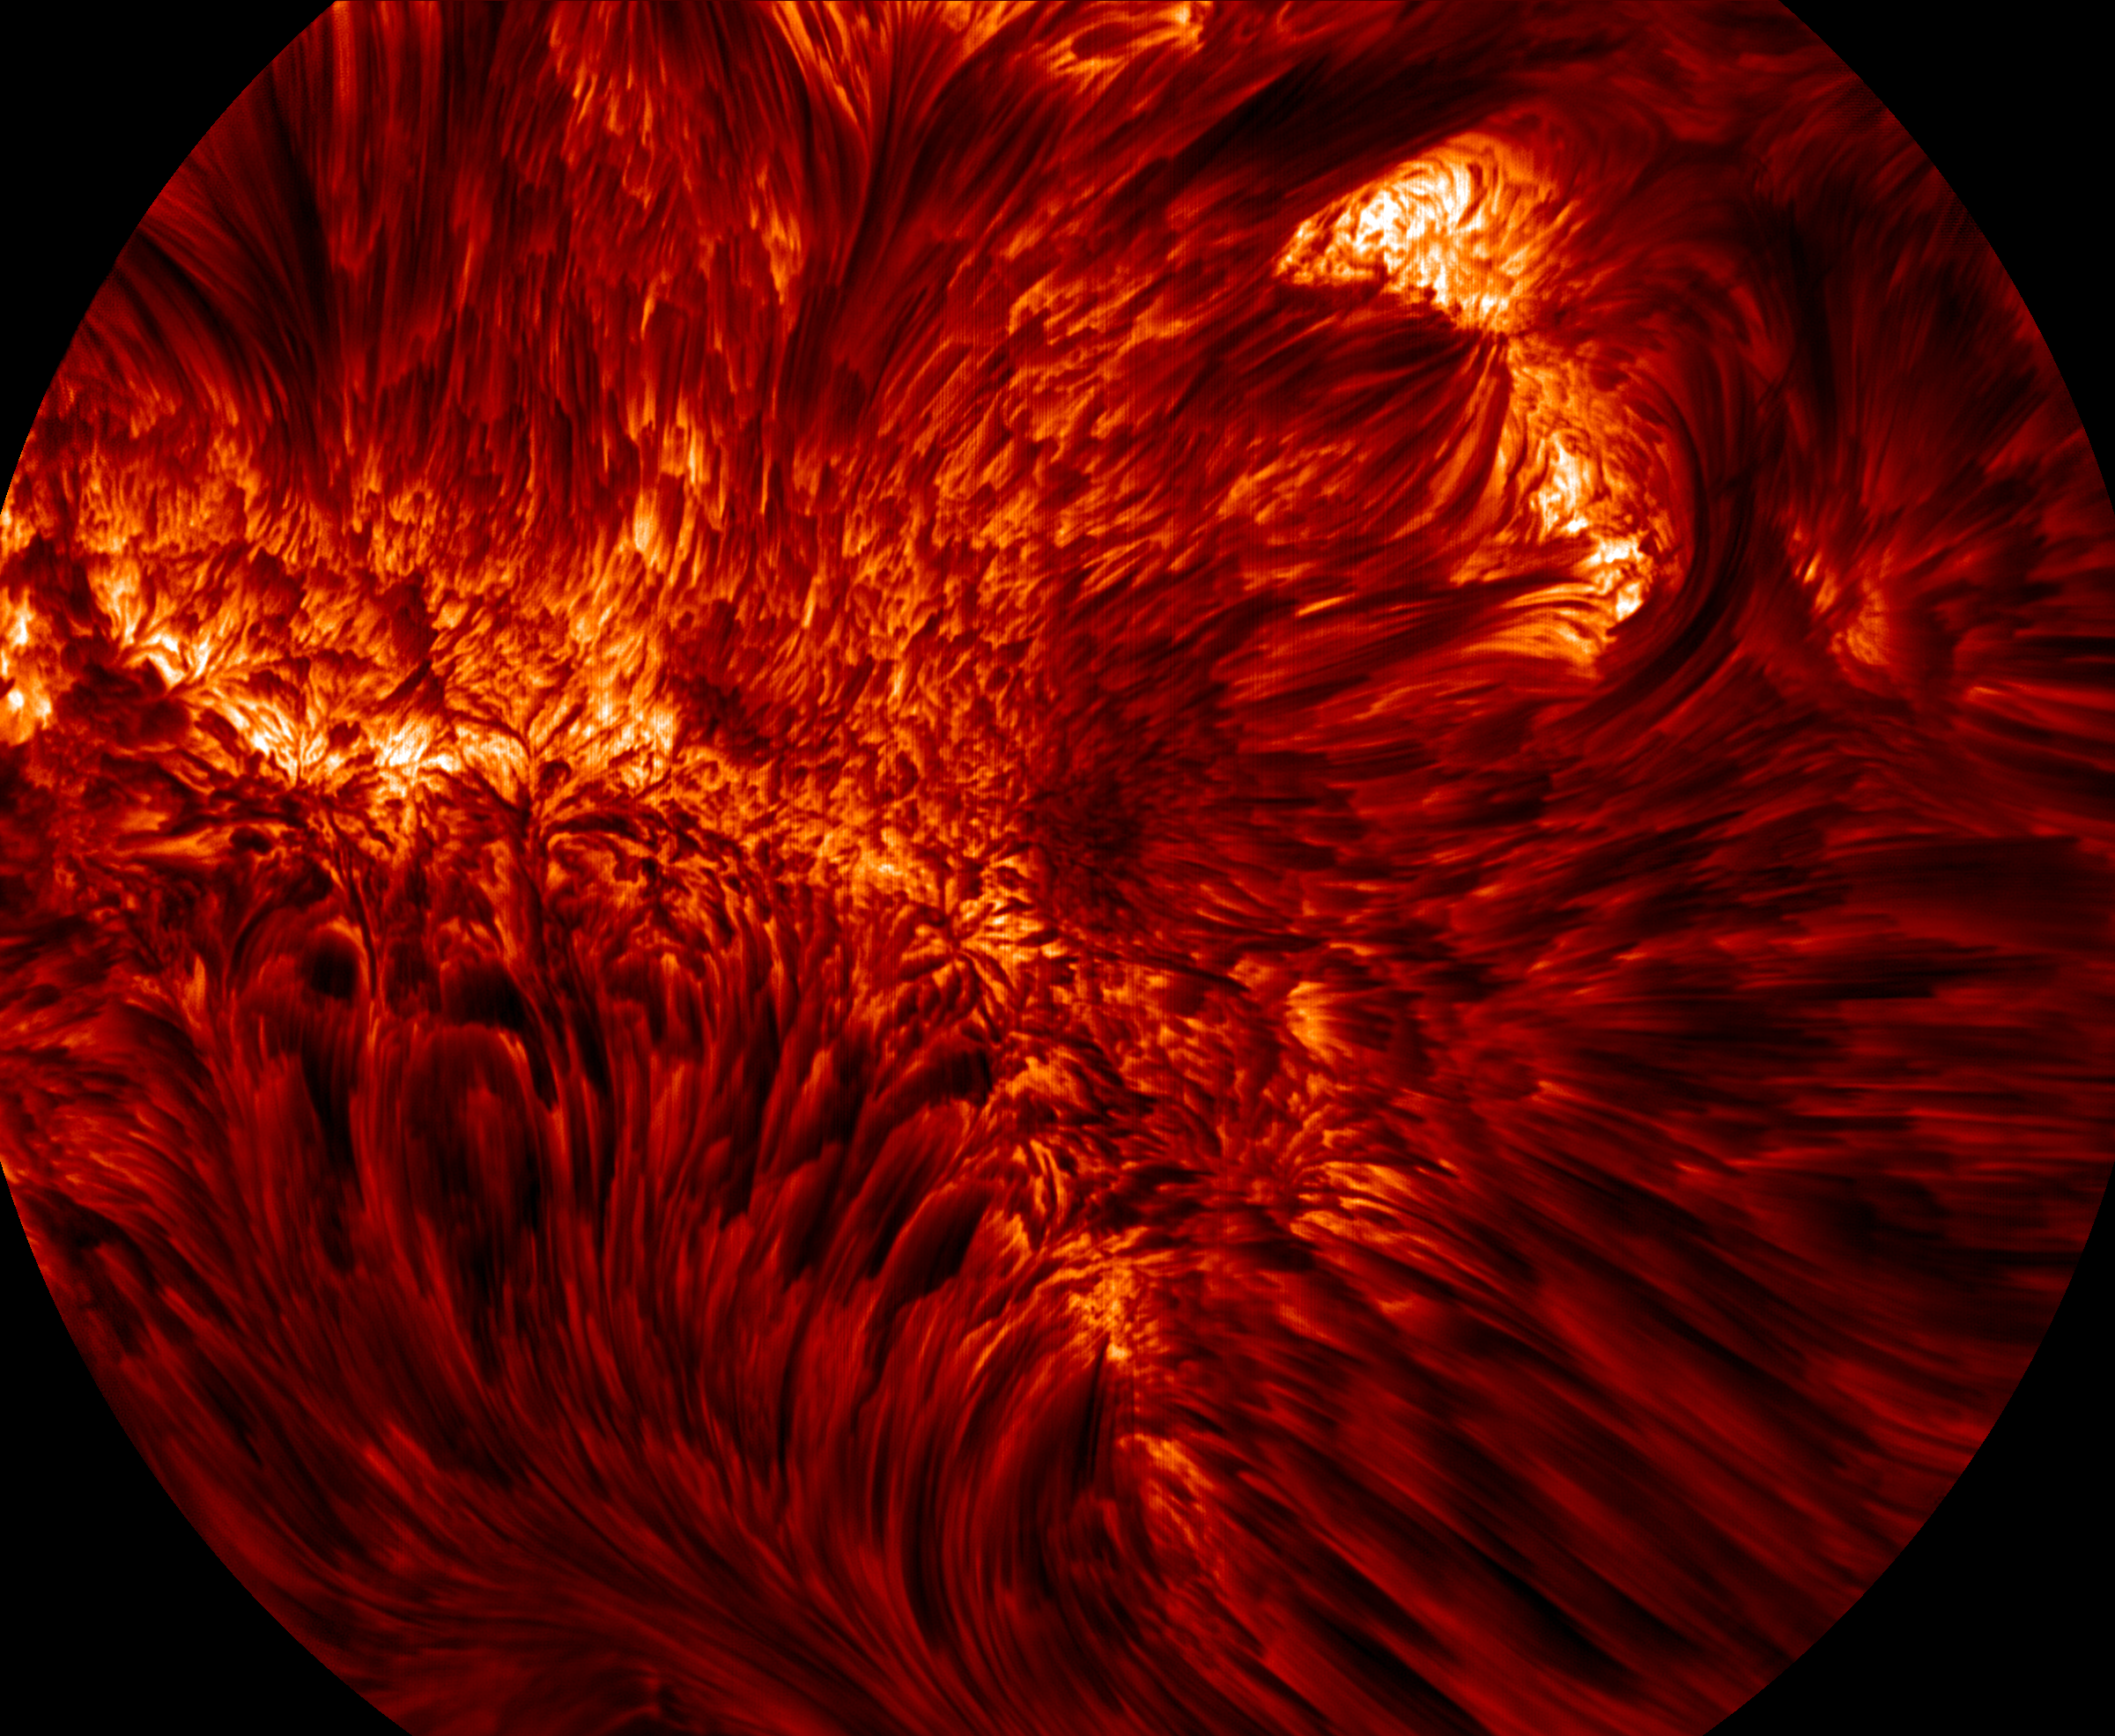
\includegraphics[scale=0.03]{chrom.png}
			\end{figure}
    \end{column}
\end{columns}

\begin{columns}[c]
    \begin{column}{0.6\textwidth}
		Corona
        \begin{itemize}
					\item magnetically dominated 
					\item very low density
					\item all ionized, MHD can be applied
        \end{itemize}
    \end{column}
    \begin{column}{0.5\textwidth}
			\begin{figure}[t]
			 \centering
			 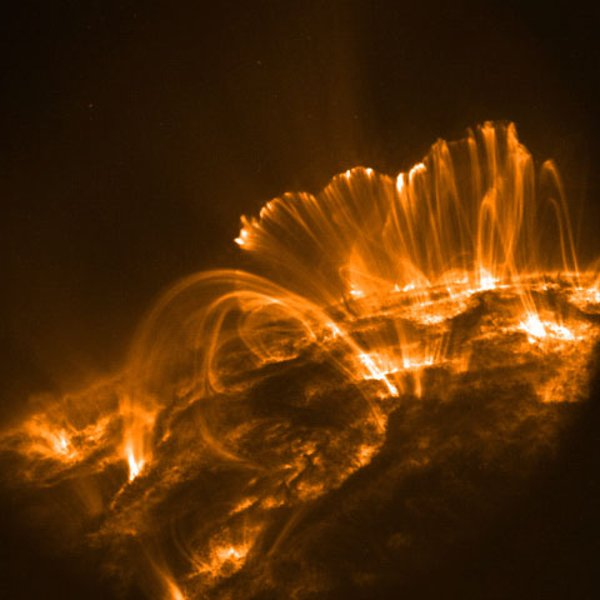
\includegraphics[scale=0.11]{corona.jpg}
			\end{figure}
    \end{column}
\end{columns}

\end{frame}


%a) Decir para que queremos 2 fluidos
%b) Poner sistema de ecuaciones de 2 fluidos que vamos a resolver. Se puede mencionar brevemente el metodo numerico, hiperdifusividades y forma que tienen los coeficientes difusivos. Pero sin entrar en detalle y poniendo referencias a trabajos publicados.
%c) Decir que lo mas problematico son los terminos colisionales
%d) Describir la forma que tienen los terminos colisionales. Aqui si podemos usar algunas formulas de la version #0, pero no todas. Hay que comparar las diferentes maneras de presentar estos terminos, comparando el paper de Leake y el nuestro. Por cierto, has conseguido derivar estos terminos a partir del documento de ecuaciones que te dimos?
%e) Decir que aproximaciones usamos (mencionar el paper de Leake et al.. y de donde vienen). Has conseguido encontrar atriculos donde derivan las formulas de Leake?
%f) Decir que no valen los metodos numericos estandar y buscamos alternativa. Dar ejemplos de lo que hacen los demas. Decir lo que haces tu.
%g) Finalizar presentando los tests

\begin{frame}{Two fluid model is needed for the chromosphere}

\begin{equation} \nonumber
\frac{\partial \rho_n}{\partial t} + \vec{\nabla} (\rho_n\vec{u}_n) = S_n
\end{equation}
%
\begin{equation} \nonumber
\frac{\partial \rho_c}{\partial t} + \vec{\nabla} (\rho_c\vec{u}_c) = -S_n
\end{equation}
%
\begin{equation}\nonumber
\frac{\partial (\rho_n\vec{u_n})}{\partial t} + \vec{\nabla}(\rho_n\vec{u_n} \otimes \vec{u_n}+{\bf\hat{p}}_n)= \rho_n\vec{g} +\vec{R}_n
\end{equation}
%
\begin{equation} \nonumber
\frac{\partial (\rho_c\vec{u_c})}{\partial t} + \vec{\nabla}(\rho_c\vec{u}_c\otimes\vec{u}_c+{\bf\hat{p}}_{c})=[\vec{J}\times\vec{B}] + \rho_c\vec{g}  -\vec{R}_n
\end{equation}
%
\begin{eqnarray} \nonumber
\frac{\partial}{\partial t} \left( e_n+\frac{1}{2}\rho_n u_n^2 \right) +  \vec{\nabla}\left( \vec{u}_n (e_n + \frac{1}{2}\rho_n u_n^2) + {\bf\hat{p}}_n\vec{u}_n + \vec{q}_{n}^{\prime} + \vec{F}_R^n \right)  = \\ \nonumber
%
\rho_n\vec{u}_n\vec{g}  + M_n
\end{eqnarray}
%
\begin{eqnarray} \nonumber
\frac{\partial}{\partial t} \left(  e_c+\frac{1}{2}\rho_c u_c^2 \right) +  \vec{\nabla}\left( \vec{u}_c (e_c + \frac{1}{2}\rho_c u_c^2) + {\bf\hat{p}}_c\vec{u}_c + \vec{q}_{c}^{\prime} + \vec{F}_R^c \right)  = \\ \nonumber
%
\rho_c\vec{u}_c\vec{g} + \vec{J}\vec{E} -M_n
\end{eqnarray}

\end{frame}

%%%%%%%%%%%%%%%%%%%%%%%%%%%%%%%%%%%%%%%%%%%%%%%%%%%%%%%%%%%%
\begin{frame}{Current assumptions}

\begin{itemize}

\item Radiation is not taken into account, $\vec{F}_R^c=\vec{F}_R^n=0$, $\vec{q}_{c}^{\prime} = \vec{q}_{c} $, $\vec{q}_{n}^{\prime} = \vec{q}_{n} $

\item Neglect pressure tensor $\hat{p}_c=p_c$, $\hat{p}_n=p_n$

\item Singly ionized Hydrogen plasma ($n_i = n_e$)

\item Ideal gas, $e_n=3p_n/2$

\item ionization energy contribution to internal energy of charges: $e_c = 3p_c/2+ n_e \phi_{ion}$

\end{itemize}

Ohm's law for the Electric field

\begin{eqnarray} \nonumber
[\vec{E} + \vec{u}_c\times{\vec{B}}] = \frac{1}{en_e}[\vec{J}\times \vec{B}] -  \frac{1}{e n_e}\vec{\nabla}{p_e} + \frac{\rho_e\nu_e}{(en_e)^2}\vec{J}  - \frac{\rho_e(\nu_{en} - \nu_{in})}{en_e}(\vec{u}_c - \vec{u}_n) 
\end{eqnarray}

\end{frame}
%%%%%%%%%%%%%%%%%%%%%%%%%%%%%%%%%%%%%%%%%%%%%%%%%%%%%%%%%%%%

\begin{frame}{Collisional terms $S_n$, $\vec{R}_n$ and $M_n$}

Obtained via momenta of the Boltzman equation

\begin{equation} \nonumber
\frac{\partial f_{\alpha} }{\partial t} + (\vec{v}\vec{\nabla})  f_{\alpha} + (\vec{a} \vec{\nabla_v} )f_{\alpha} = \left (\frac{\partial f_{\alpha}}{\partial t} \right )_{\rm coll} \stackrel{\text{not}}{=} C_\alpha 
\end{equation}

with $\alpha \in {i,e,n}$ (charges, c = e+i)
%
\begin{equation} \nonumber
S_{\alpha}=m_{\alpha}\int_{V}{\left(\frac{\partial f_{\alpha}}{\partial t}\right)_{\rm coll} d^3 v} = \left( \frac{\partial \rho_{\alpha}}{\partial t} \right)_{\rm coll} 
\end{equation}

\begin{equation} \nonumber
\vec{R}_{\alpha}=m_{\alpha}\int_V{\vec{v}\left(\frac{\partial f_{\alpha}}{\partial t}\right)_{\rm coll}d^3 v} = \left( \frac{\partial}{\partial t}
[\rho_{\alpha}\vec{u}_{\alpha}] \right)_{\rm coll}
\end{equation}


\begin{equation} \nonumber
M_{\alpha}=\frac{1}{2} m_{\alpha} \int_V{v^2\left(\frac{\partial f_{\alpha}}{\partial t}\right)_{\rm coll} d^3 v} = \left( \frac{\partial }{\partial t} [\frac{1}{2}\rho_{\alpha} u_{\alpha}^2] \right)_{\rm coll}  +
\left( \frac{\partial }{\partial t} [\frac{3}{2}p_{\alpha}] \right)_{\rm coll}
\end{equation}

\end{frame}
%%%%%%%%%%%%%%%%%%%%%%%%%%%%%%%%%%%%%%%%%%%%%%%%%%%%%%%%%%%%

\begin{frame}{Collisional terms }

\begin{equation} \nonumber
C_{\alpha} = C_\alpha^{\rm inelastic}  + C_\alpha^{\rm elastic} = \sum_{\alpha'} {(n_{\alpha'} C_{\alpha'\alpha}^{\rm inelastic} - n_{\alpha} C_{\alpha\alpha'}^{\rm inelastic}}) + \sum_{\beta} C_{\alpha \beta}^{\rm elastic}
\end{equation}

\begin{equation}  \nonumber
C_{\alpha\alpha'}^{\rm inelastic} =  \sum_{\beta} {C_{\alpha\alpha',\beta}^{\rm inelastic} } = \sum_{\beta} \sigma_{\alpha \alpha'} (v_{\beta})f_{\beta} v_{\beta}
\end{equation}

where $\sigma_{\alpha \alpha'} = \sigma_{\alpha \alpha'}(v_{\beta}) $  is the collisional cross section of $\alpha$ and $\beta$ 
\vspace{0.5cm}

{\bf Inelastic collisions: ionization and recombination processes} 
\vspace{0.5cm}


In our case, we need to know only $C_n$ for hydrogen plasma

\begin{equation}  \nonumber
C_n^{\rm inelastic} = n_i  [\sigma_{in} (v_e) f_e v_e ]- n_n [\sigma_{ni} (v_e)  f_e v_e] = n_i C^{\rm rec} - n_n C^{\rm ion}
\end{equation}

\end{frame}
%%%%%%%%%%%%%%%%%%%%%%%%%%%%%%%%%%%%%%%%%%%%%%%%%%%%%%%%%%%%

\begin{frame}{Expressions for the collisional term $S_n$, inelastic}

\begin{equation} \nonumber
S_n=S_n^{\rm elastic} + S_n^{\rm inelastic}; \,\,\,\, S_n^{\rm elastic}=0
\end{equation}


\begin{equation} \nonumber
S_n=\rho_i n_e \langle \sigma_{in} (v_e) v_e\rangle - \rho_n n_e \langle \sigma_{ni} (v_e) v_e\rangle =   \rho_i \Gamma^{\rm rec} - \rho_n\Gamma^{\rm ion}
\end{equation}

approximate expressions for $\Gamma^{\rm rec}$ and $\Gamma^{\rm ion}$ are given by Voronov (1997) Leake et al. (2012)

\begin{equation} \nonumber
\Gamma^{\rm ion} = n_e \langle  \sigma_{ni} (v_e)  v_e \rangle \approx \frac{n_e}{\sqrt{T_e^*}}	2.6 \cdot 10^{-19}; \,\,\,\, {\rm s^{-1}}
\end{equation}

\begin{equation} \nonumber
\Gamma^{\rm rec} =n_e \langle  \sigma_{in} (v_e)  v_e \rangle \approx n_e A \frac{1}{X + \phi_{\rm ion}/{T_e^*}}\left(\frac{\phi_{\rm ion}}{T_e^*}\right)^K  e^{-\phi_{\rm ion}/T_e^*}; \,\,\,\,  {\rm s^{-1}}
\end{equation}

$\phi_{\rm ion} = 13.6 eV$

$T_e^*$ is electron temperature in eV

$A = 2.91 \cdot 10^{-14}$

$K = 0.39, X = 0.232$

\end{frame}
%%%%%%%%%%%%%%%%%%%%%%%%%%%%%%%%%%%%%%%%%%%%%%%%%%%%%%%%%%%%

\begin{frame}{Expressions for the term $\vec{R}_n$, elastic \& inelastic}

{\small
\begin{equation} \nonumber
\vec{R}_n=\vec{R}_n^{\rm elastic} + \vec{R}_n^{\rm inelastic}
\end{equation}
since $v_\alpha = u_\alpha + c_\alpha$ (macroscopic and random velocity)

Momentum added/removed by ionizing and recombining particles via inelastic collisions
\begin{eqnarray} \nonumber
\vec{R}_{\alpha\alpha',\beta}^{\rm inelastic} = m_\alpha \int_V{\vec{v}_\alpha \sigma_{\alpha \alpha'} f_{\beta} v_{\beta} d^3\vec{v} } = \vec{u}_\alpha S_{\alpha\alpha',\beta}^{\rm inelastic}    
\end{eqnarray}

\begin{equation} \nonumber
\vec{R}_n^{\rm inelastic} = \rho_i \vec{u}_i \Gamma^{rec} - \rho_n \vec{u}_n \Gamma^{ion} 
\end{equation}

Momentum added/removed via elastic collisions
\begin{eqnarray}  \nonumber
\vec{R}_\alpha^{\rm elastic} = m_\alpha \int_V{v_\alpha C_\alpha^{\rm elastic} d^3\vec{v} } = m_\alpha \int_V{c_\alpha C_\alpha^{\rm elastic} d^3\vec{v} } 
\end{eqnarray}

\begin{eqnarray}  \nonumber
\vec{R}_n^{\rm elastic}  = -\rho_e(\vec{u}_n - \vec{u}_e) \nu_{en} - \rho_i(\vec{u}_n - \vec{u}_c) \nu_{in}
\end{eqnarray}

expressed in terms of current $\vec{J}$
\begin{eqnarray} \nonumber
\vec{R}_n^{\rm elastic} = (\rho_e\nu_{en} + \rho_i\nu_{in})(\vec{u}_c - \vec{u}_n) - \frac{\vec{J}}{en_e}\rho_e\nu_{en}
\end{eqnarray}

}

\end{frame}
%%%%%%%%%%%%%%%%%%%%%%%%%%%%%%%%%%%%%%%%%%%%%%%%%%%%%%%%%%%%

\begin{frame}{Expressions for the term $M_n$, elastic \& inelastic }

\begin{equation} \nonumber
M_n= M_n^{\rm elastic} + M_n^{\rm inelastic}
\end{equation}

Generically

\begin{equation} \nonumber
M_{\alpha\alpha',\beta}^{\rm inelastic} = \frac{1}{2} m_\alpha \int_V{v_\alpha^2 \sigma_{\alpha \alpha'} f_{\beta} v_{\beta} d^3\vec{v} } = 
\frac{1}{2} u_\alpha^2 S_{\alpha\alpha',\beta}^{\rm inelastic} + \frac{3 k_B T_\alpha}{2 m_\alpha} S_{\alpha\alpha',\beta}^{\rm inelastic} 
\end{equation}

In our particular case,

\begin{equation} \nonumber
M_n^{\rm inelastic} = \frac{1}{2} \rho_i u_i^2 \Gamma^{\rm rec} - \frac{1}{2}\rho_n u_n^2 \Gamma^{\rm ion} + \frac{3}{2} k_B\left ( \frac{\rho_i T_i}{m_i} \Gamma^{\rm rec} - \frac{\rho_n T_n}{m_n} \Gamma^{\rm ion} \right)
\end{equation} 

\begin{equation} \nonumber
M_\alpha^{\rm elastic} = \frac{1}{2} m_\alpha \int_V{v_\alpha^2 C_\alpha^{\rm elastic} d^3\vec{v} } = \vec{u}_\alpha \vec{R}_\alpha^{\rm elastic} + \frac{1}{2} m_\alpha \int_V{c_\alpha^2 C_\alpha^{\rm elastic} d^3\vec{v} } 
\end{equation} 

The second term is neglected for the moment

\begin{equation}  \nonumber
M_n^{\rm elastic} = \vec{u}_n \vec{R}_n^{\rm elastic} ; \,\,\,\,M_c^{\rm elastic} = -\vec{u}_c \vec{R}_n^{\rm elastic}
\end{equation}

\end{frame}
%%%%%%%%%%%%%%%%%%%%%%%%%%%%%%%%%%%%%%%%%%%%%%%%%%%%%%%%%%%%
\begin{frame}{Equilibrium atmosphere and perturbaion}


{\sc Mancha} {\bf code separates variables for equilibrium and perturbation. 
One needs to provide an equilibrium atmosphere.}


\begin{itemize}
\item 13 variables: 10 variables p , $\rho$ and $\vec{u}$ of the 2 fluids: charges(\_c) and neutrals(\_n) + magnetic field
\item hydrostatic equilibrium (variables: $p_{c0}, p_{n0}, \rho_{c0}, \rho_{n0}$, $\vec{B_0}$), $\vec{u_{c0}}=\vec{u_{n0}}=0$
 
\begin{itemize}
\item charges:
\begin{equation}
\rho_{c0}\vec{g} - \vec{\nabla} p_{c0} + \frac{1}{\mu_0} (\nabla \times \vec{B_0}) \times \vec{B_0} = 0
\end{equation}

\item neutrals:
\begin{equation}
\rho_{n0}\vec{g} - \vec{\nabla} p_{n0}  = 0
\end{equation}

\end{itemize}
\item 13 partial differential equations for the evolution of the perturbation (variables: $p_{c1},p_{n1}, \vec{u}_{c1},\vec{u}_{n1},\rho_{c1}, \rho_{n1}, \vec{B_1}$)

\end{itemize}

\end{frame}

%%%%%%%%%%%%%%%%%%%%%%%%%%%%%%%%%%%%%%%%%%%%%%%%%%%%%%%%%%%%
\begin{frame} {Momentum equation, numerical treatment of stiff collisional terms}

\begin{equation}\nonumber
\frac{\partial (\rho_n\vec{u_n})}{\partial t} + \vec{\nabla}(\rho_n\vec{u_n} \otimes \vec{u_n}+p_n)= \rho_n\vec{g} +\vec{R}_n
\end{equation}
%
\begin{equation} \nonumber
\frac{\partial (\rho_c\vec{u_c})}{\partial t} + \vec{\nabla}(\rho_c\vec{u}_c\otimes\vec{u}_c+p_{c})=[\vec{J}\times\vec{B}] + \rho_c\vec{g}  -\vec{R}_n
\end{equation}

Using the method from Smith \& Sakai (2008)

the first term in $\vec{R}_n^{\rm elastic}$: $(\rho_e\nu_{en} + \rho_i\nu_{in})(\vec{u}_c - \vec{u}_n)$ written as  

$\rho_c \rho_n \alpha (\vec{u}_c - \vec{u}_n)  $ with
 
\begin{equation} \nonumber
\alpha = \frac{1}{m_n^2} \left (\sqrt{\frac{8 k_B T_{nc}}{\pi m_{in}}} m_{in} \Sigma_{in} +  \sqrt{\frac{8 k_B T_{nc}}{\pi m_{en}}} m_{en} \Sigma_{en} \right ) 
\end{equation}

is calculated as 

\begin{equation} \nonumber
\frac{\rho_c \rho_n \alpha dt}{1 + \alpha(\rho_c + \rho_n) dt }(\vec{u}_c - \vec{u}_n)
\end{equation}

\end{frame}

%%%%%%%%%%%%%%%%%%%%%%%%%%%%%%%%%%%%%%%%%%%%%%%%%%%%%%%%%%%%

\begin{frame}{Orszag test}
extended from mancha 1 fluid test

no collision terms, variable artificial diffusivity and filtering

\textbf{Initial conditions}:

with:
  $scale_v = 10^{-2}$,
  $scale_b = 10^{-4}$,
  $scale_p = 10^{-1}$,
  $scale_\rho = 10^{3}$,
  $scale_d = 10^{-2}$,
	$L = 1.0  scale_d$,
	$A=0.2$

{\bf Equilibrium}

$\rho_{c00} = \frac{25}{36 \pi} scale_\rho$,
$p_{c00} =  \frac{5}{12 \pi}   scale_p$

$\rho_{n00} = \rho_{c00}$,
$p_{n00} = \frac{1}{2} pe_{c00}$,


{\bf Perturbation}

${u_c}_x = -(1 + A \sin(\frac{2 \pi z}{L}))  \sin(\frac{2 \pi y}{L}) scale_v$,
${u_c}_y = (1 + A \sin(\frac{2 \pi z}{L}))  \sin(\frac{2 \pi x}{L}) scale_v$,
${u_c}_z =  A \sin(\frac{2 \pi z}{L}))  scale_v$,
$\vec{u}_n = \vec{u}_c$

$B_x = -\sin(\frac{2\pi y}{L}) scale_b$,
$B_y =  \sin(\frac{4\pi x}{L}) scale_b$,
$B_z = 0$



resolution: 128x128x128 points

\end{frame}

%%%%%%%%%%%%%%%%%%%%%%%%%%%%%%%%%%%%%%%%%%%%%%%%%%%%%%%%%%%%

\begin{frame}{Orszag test}

\begin{figure}[H]
 \centering
 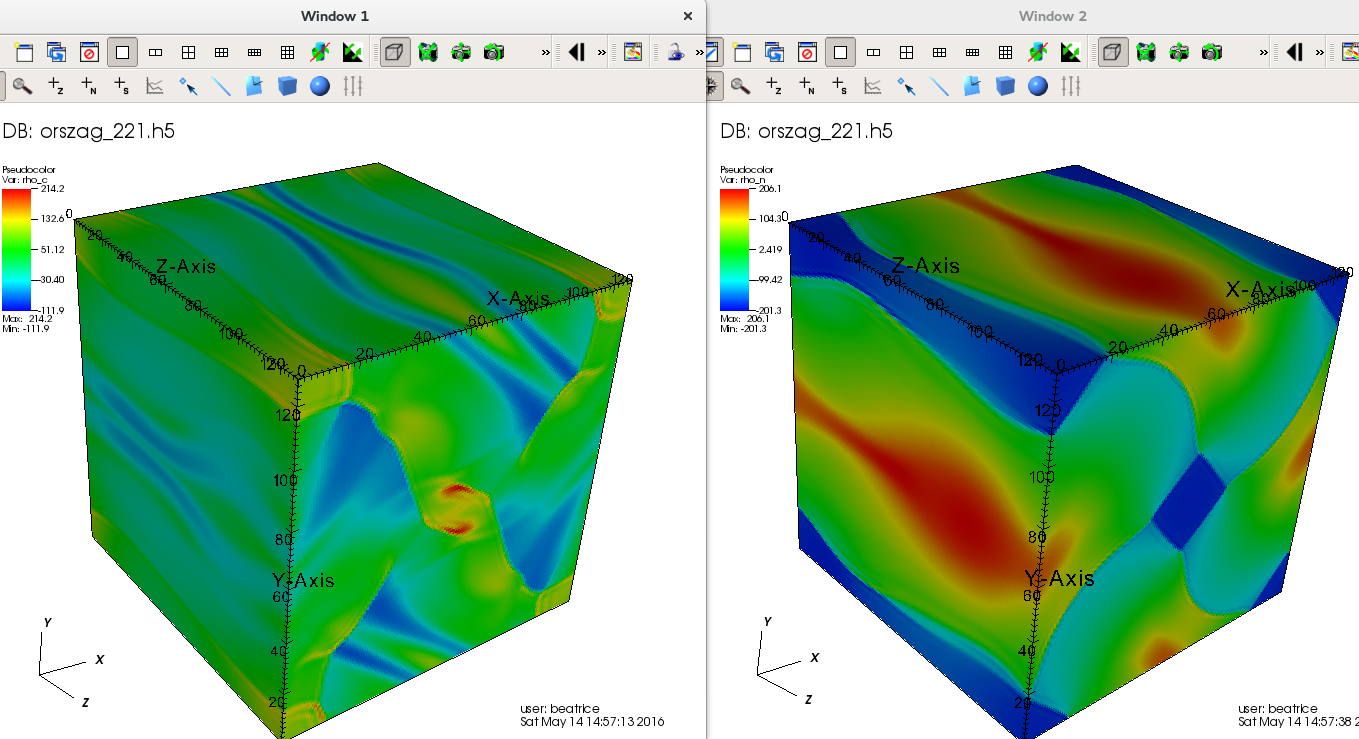
\includegraphics[scale=0.24]{visit2.png}
  \caption{density of charges and neutrals in Orszag test after 0.3836 s (221 iterations) where they evolve independently (collision terms between neutrals and charges are set to 0)}
\end{figure}
\end{frame}
%%%%%%%%%%%%%%%%%%%%%%%%%%%%%%%%%%%%%%%%%%%%%%%%%%%%%%%%%%%%

\begin{frame}{Acoustic Wave}
extended from mancha 1 fluid test

\textbf{Initial conditions}:

\textbf{hydrostatic equilibrium} in an isothermal gravity stratified atmosphere:

$\vec{B_0}=(0,0,B_{z0})$, $B_{z0} = 50 \cdot 10^{-4}$ T, $\nabla \times \vec{B_0} = 0$

$\frac{\partial p_\alpha}{\partial z} = -\rho_\alpha  g$

we define total pressure at the  base  $p_{00}= p_0(z=0)=1.17 \cdot 10^4$ Pa  and uniform temperature equal for neutrals and charges: $T_0=10000$ K

assuming hydrogen plasma we calculate from Saha equation the pressure of neutrals and charges at the base: $p_{n00}$, $p_{c00}$

we have different pressure scale heights for charges and neutrals: $H_\alpha = \frac{R T_0}{\mu_\alpha g}$ beacuse of different $\mu_c=\frac{1}{2} \mu_n$  and $\mu_n = 1g/mol$ (only H)

we calculate then equilibrium pressure of charges and neutrals: $p_{\alpha0}(z) = p_{\alpha00} \exp(-\frac{z}{H_\alpha})$

and density from ideal gas law: $\rho_{\alpha0} = \frac{p_{\alpha0} \mu_\alpha}{R T_0}$
\end{frame}


%%%%%%%%%%%%%%%%%%%%%%%%%%%%%%%%%%%%%%%%%%%%%%%%%%%%%%%%%%%%


\begin{frame}{Acoustic Wave}

\textbf{perturbation} - a gaussian shaped(in the xy plane) sound wave generated permanently(time condition) at the base of the gravity stratified atmosphere:

defining  A=100, the period P=50  ($\omega=\frac{2 \pi}{P}$) of the wave, $x_0$, $y_0$, $\sigma_x$, $\sigma_y$ the center and the standard deviation of the gaussian and
 $z_f$ the end of the perturbed region 

the cutoff frequency: ${\omega_c}_\alpha = \frac{\gamma g}{2 {c_s}_\alpha}$

the pressure scale height: $H_\alpha=\frac{{{c_s}_\alpha}^2}{\gamma g}$


\[
k_\alpha=
 \begin{cases} 
      -\frac{\sqrt{\omega^2 - {\omega_c}_\alpha^2}}{{c_s}_\alpha} - \frac{i}{2 H_\alpha}& \omega \ge {\omega_c}_\alpha \\
      i(\frac{\sqrt{\omega^2 - {\omega_c}_\alpha^2}}{{c_s}_\alpha} - \frac{1}{2 H_\alpha})& \omega < {\omega_c}_\alpha 
   \end{cases}
\]

$g(x,y) = exp(-\frac{(x-x_0)^2}{2 \sigma_x^2} -\frac{(y-y_0)^2}{2 \sigma_y^2} )$

$rr_\alpha = \frac{1}{\omega}(-k_\alpha - \frac{i}{H_\alpha})$

$pp_\alpha = \frac{1}{\omega}(-k_\alpha \gamma - \frac{i}{H_\alpha})$

\end{frame}


%%%%%%%%%%%%%%%%%%%%%%%%%%%%%%%%%%%%%%%%%%%%%%%%%%%%%%%%%%%%


\begin{frame}{Acoustic Wave}
\begin{eqnarray} \nonumber
p_{\alpha1}(x,y,z,t) = A \cdot g(x,y) \cdot {p_{\alpha0}} \cdot|pp_\alpha| \cdot \exp \left [Im(k_\alpha) (z_f - z) \right ] \\ 
\sin \left [ Re(k_\alpha) (z_f - z) + \omega t + atan \left (\frac{Im(pp_\alpha)}{Re(pp_\alpha)} \right ) \right ]
\end{eqnarray}

\begin{eqnarray} \nonumber
\rho_{\alpha1}(x,y,z,t) = A \cdot g(x,y) \cdot {\rho_{\alpha0}} \cdot|rr_\alpha| \cdot \exp \left [Im(k_\alpha) (z_f - z) \right ] \\ 
\sin \left [ Re(k_\alpha) (z_f - z) + \omega t + atan \left (\frac{Im(rr_\alpha)}{Re(rr_\alpha)} \right ) \right ]
\end{eqnarray}

\begin{eqnarray} \nonumber
u_{\alpha1}(x,y,z,t) = A \cdot g(x,y) \cdot  \exp \left [Im(k_\alpha) (z_f - z) \right ] \\ \sin \left [ Re(k_\alpha) (z_f - z) + \omega t  \right ]
\end{eqnarray}


in this test we used a Perfectly Matched Layer to avoid reflection at the upper boundary (described in previous version of Mancha) 



\end{frame}




%%%%%%%%%%%%%%%%%%%%%%%%%%%%%%%%%%%%%%%%%%%%%%%%%%%%%%%%%%%%



\begin{frame}{Acoustic Wave}
for $\Gamma^{\rm ion}$ and $\Gamma^{\rm rec}$ instead of expression from Leake the derivation of Saha equation in time (only derivating T and not $n_{tot}$):

\begin{eqnarray} \nonumber
\frac{\partial n_e}{\partial t} = 
\left (\frac{2  \pi  m_e  k_B}{h^2} \right )^{1.5} \exp \left (-\frac{\phi_{ion}} {k_B T_{cn}} \right )
      \left (1.5  \sqrt{T_{cn}}  + \frac{\phi_{ion}}{k_B T_{cn}^2 } \right) \\ 
     \left ( \frac{2 A+ n_{tot}}{2 \sqrt{A^2 + A n_{tot}} } - 1 \right)\frac{\partial T_{cn}}{\partial t} 
       min \left (\frac{dt}{\tau_{rel}},1 \right )
\end{eqnarray}

				where $A = \left (\frac{2  \pi  m_e  k_B  T_{cn}}{h^2} \right )^{1.5}  \exp \left (-\frac{\phi_{ion}} { k_B  T_{cn}} \right)$

and the relaxation timescale for saha $\tau_{rel}$ is a  parameter set to 10 in this test

     where($\frac{\partial n_e}{\partial t} <0$) $\Gamma^{\rm rec} = -\frac{m_H}{\rho_c}  \frac{\partial n_e}{\partial t} $, $\Gamma^{\rm ion} = 0 $

     elsewhere $\Gamma^{\rm ion} = \frac{m_H}{\rho_n} \frac{\partial n_e}{\partial t} $, $\Gamma^{\rm rec} = 0 $

\end{frame}


%%%%%%%%%%%%%%%%%%%%%%%%%%%%%%%%%%%%%%%%%%%%%%%%%%%%%%%%%%%%


\begin{frame}{Reconnection}

Initial conditions from Leake article

defining:
$L_0 =10^{5}$,
$n_0 = 3.3\cdot 10^{16}$,
$B_0 = 10^{-3}$, 
$v_0 = 1.2\cdot 10^5$, 
$T_0 = 1.75\cdot 10^6$, 
$P_0 = 0.8$,
$L_p = 0.5  L_0$,
$F = 0.01  P_0$
$y_s = 0.5 L_y$,
$x_s = 0.5 L_x$

domain size:
$L_x = 72 L_0$,
$L_y = 12 L_0$;
resolution: 256x256x1

including all terms of plasma diffusivity (in Ohm law)  and artificial diffusivity (variable and constant)

{\bf equilibrium:}

${n_n}_0 = 200 n_0$,
${n_i}_0 = {n_e}_0 = n_0$, 
$T_{00} = 0.005  T_0$ (for both c and n)


{\bf perturbation:}

$pe_{c1} = 0.5 \frac{ F}{ (cosh \left( \frac{y-y_s}{L_p} \right ))^2}$

$pe_{n1} = 0.5 \frac{1-F} { (cosh \left( \frac{y-y_s}{L_p} \right ))^2}$


\end{frame}




%%%%%%%%%%%%%%%%%%%%%%%%%%%%%%%%%%%%%%%%%%%%%%%%%%%%%%%%%%%%



\begin{frame}{Reconnection}


with velocity:

$v_{\delta0} = 5 \cdot 10^{-4}  v_0$

$rr = \left( \frac{ (\frac{x-x_s}{5})^2 + (y-y_s)^2}{L_p^2} \right )^2$

$v_{1x} = v_{\delta0}  \sin \left ( \frac{x-x_s}{5 L_p} \right ) \left (\cos( \frac{y-y_s}{L_p}) - \frac{2(y-y_s)}{L_p} \sin ( \frac{y-y_s}{L_p}) \right) \exp(-rr)$

$v_{1y} = -\frac{v_{\delta0}}{5}  \sin \left ( \frac{y-y_s}{L_p} \right ) \left (\cos( \frac{x-x_s}{5 L_p}) - \frac{2(x-x_s)}{5 L_p} \sin ( \frac{x-x_s}{5 L_p}) \right) \exp(-rr)$



${u_c}_y = \frac{ (F-1)n_0^2 v_0^2}{{n_i}_0 {n_n}_0 \nu_{in}  L_p}  \frac{tanh (\frac{y-y_s}{L_p}) } {(cosh(\frac{y-y_s}{L_p}))^2}+ v_{1y}$,
where 
$\nu_{in} = {n_n}_0 \cdot 1.41 \cdot 10^{-19} \sqrt{ \frac{8 k_B T_{00}}{\pi m_{ih}}} $

${u_c}_x = v_{1x}$,
${u_n}_x = v_{1x}$,
${u_n}_y = v_{1y}$


$A = \frac{0.01  B_0  L_0}{ L_p^2}  \exp \left(-( \frac{x-x_s}{4 L_p})^2 \right )  \exp \left (-( \frac{y-y_s}{L_p})^2 \right)$

$B_{1x} = -B_0  tanh ( \frac{y-y_s}{L_p}) +2 A  (y-y_s)$

$B_{1y} = -\frac{A}{8}  (x-x_s) $




\end{frame}




%%%%%%%%%%%%%%%%%%%%%%%%%%%%%%%%%%%%%%%%%%%%%%%%%%%%%%%%%%%%



\begin{frame}{References}


{\small
\begin{itemize}

\item E. Khomenko,  M. Collados,  A. Dı́az and N. Vitas - Fluid description of multi-component solar partially ionized plasma

\item E. T. Meier  and U. Shumlak - A general nonlinear fluid model for reacting plasma-neutral mixtures

\item James E. Leake , Vyacheslav S. Lukin  , Mark G. Linton  and Eric T. Meier - Multi-fluid simulations of chromospheric magnetic reconnection
in a weakly ionized reacting plasma

\item James E. Leake,   Vyacheslav S. Lukin, Mark G. Linton - Magnetic Reconnection in a Weakly Ionized Plasma

\item P. D. Smith, J. I. Sakai - Chromospheric magnetic reconnection: two-fluid
simulations of coalescing current loops

\item Matts Carlsson and R.F. Stein - Dynamic Hydrogen Ionization

\item Ondas MHD en la fotosfera y
cromosfera de manchas solares - 
Memoria que presenta
Tob\'ias Felipe Garc\'ia
para optar a la titulaci\'on
de Doctor en Astrof\'isica.

\end{itemize}
}
\end{frame}
\end{document}
